\chapter{Conclusion}
\label{chap:conclusion}

\section{Conclusion}
\label{sec:conclusion}

The development of this setup was meant to be general and be used in both
research and academic environments. The process of implementing this setup went
through a myriad of fields in telecommunications and embedded systems, such as
communication protocols, embedded programming, electronics and many others,
being this setup a testbed for more complex processes inside the LTE band saves
a lot of time in development. \\

The FMComms2 board allows real-time and scalable change in parameters by
software or hardware signals, and it re-calibrates and reconfigures itself if
needed so, which makes a very good transceiver board to be used in a C-RAN
environment.\\

This setup was extensively documented and can be used in digital communication
classes to show how a real radio frontend system is made, of course there is
much to improve, there is no dynamic clock synchronization between the FPGA and
the FMComms2, there is no communication protocol between the FPGA (BBP) and the
external world other than the FMComms2 such things are necessary to have a real
frontend but were outside the scope of this project which was just to evaluate a
setup for a scalable and dynamically configurable frontend.\\

Although the FMComms2 and the FPGA operates on different clocks, thus no real
synchronization was implemented, this setup has the minimal capability of
transmitting and receiving signals and reconfigure itself on real-time, the main
goal of this work was reached, however there is much to explore with these tools
and devices.

\section{Future Works}
\label{sec:futurew}

Having finished this part of the work a natural sequel would be implementing
Ethernet connection driver in the FPGA, making it possible to receive data from
Ethernet and hand this to the transceiver board following the schematic on
figure \ref{fig:setupeth} idea. This would be a challenge because there is a lot
of things to consider, but the most problematic of them all is synchronization,
the clock in which everything inside the FPGA works is different from the AD9361
clock not only in frequency but in phase, this can bring a lot of problems,
however there is the possibility of feeding FMComms2 with an external clock
which would increase its performance.\\

With Ethernet it would be possible to generate the modulated samples and send
them trough air, just like Gnuradio + USRP and thus demodulate the received back
samples in the PC, however there is another possibility, modulation and
demodulation blocks implemented in the FPGA logic, thus much faster than the PC
ones and with partial reconfiguration there is the advantage of loading various
schemes of modulation/demodulation in the FPGA, implementing thus a very good
SDR. The Ethernet connection, is also very interesting for C-RAN
environment, because Ethernet is cheap and easy to implement.\\

\begin{figure}[htbp]
    \centering
    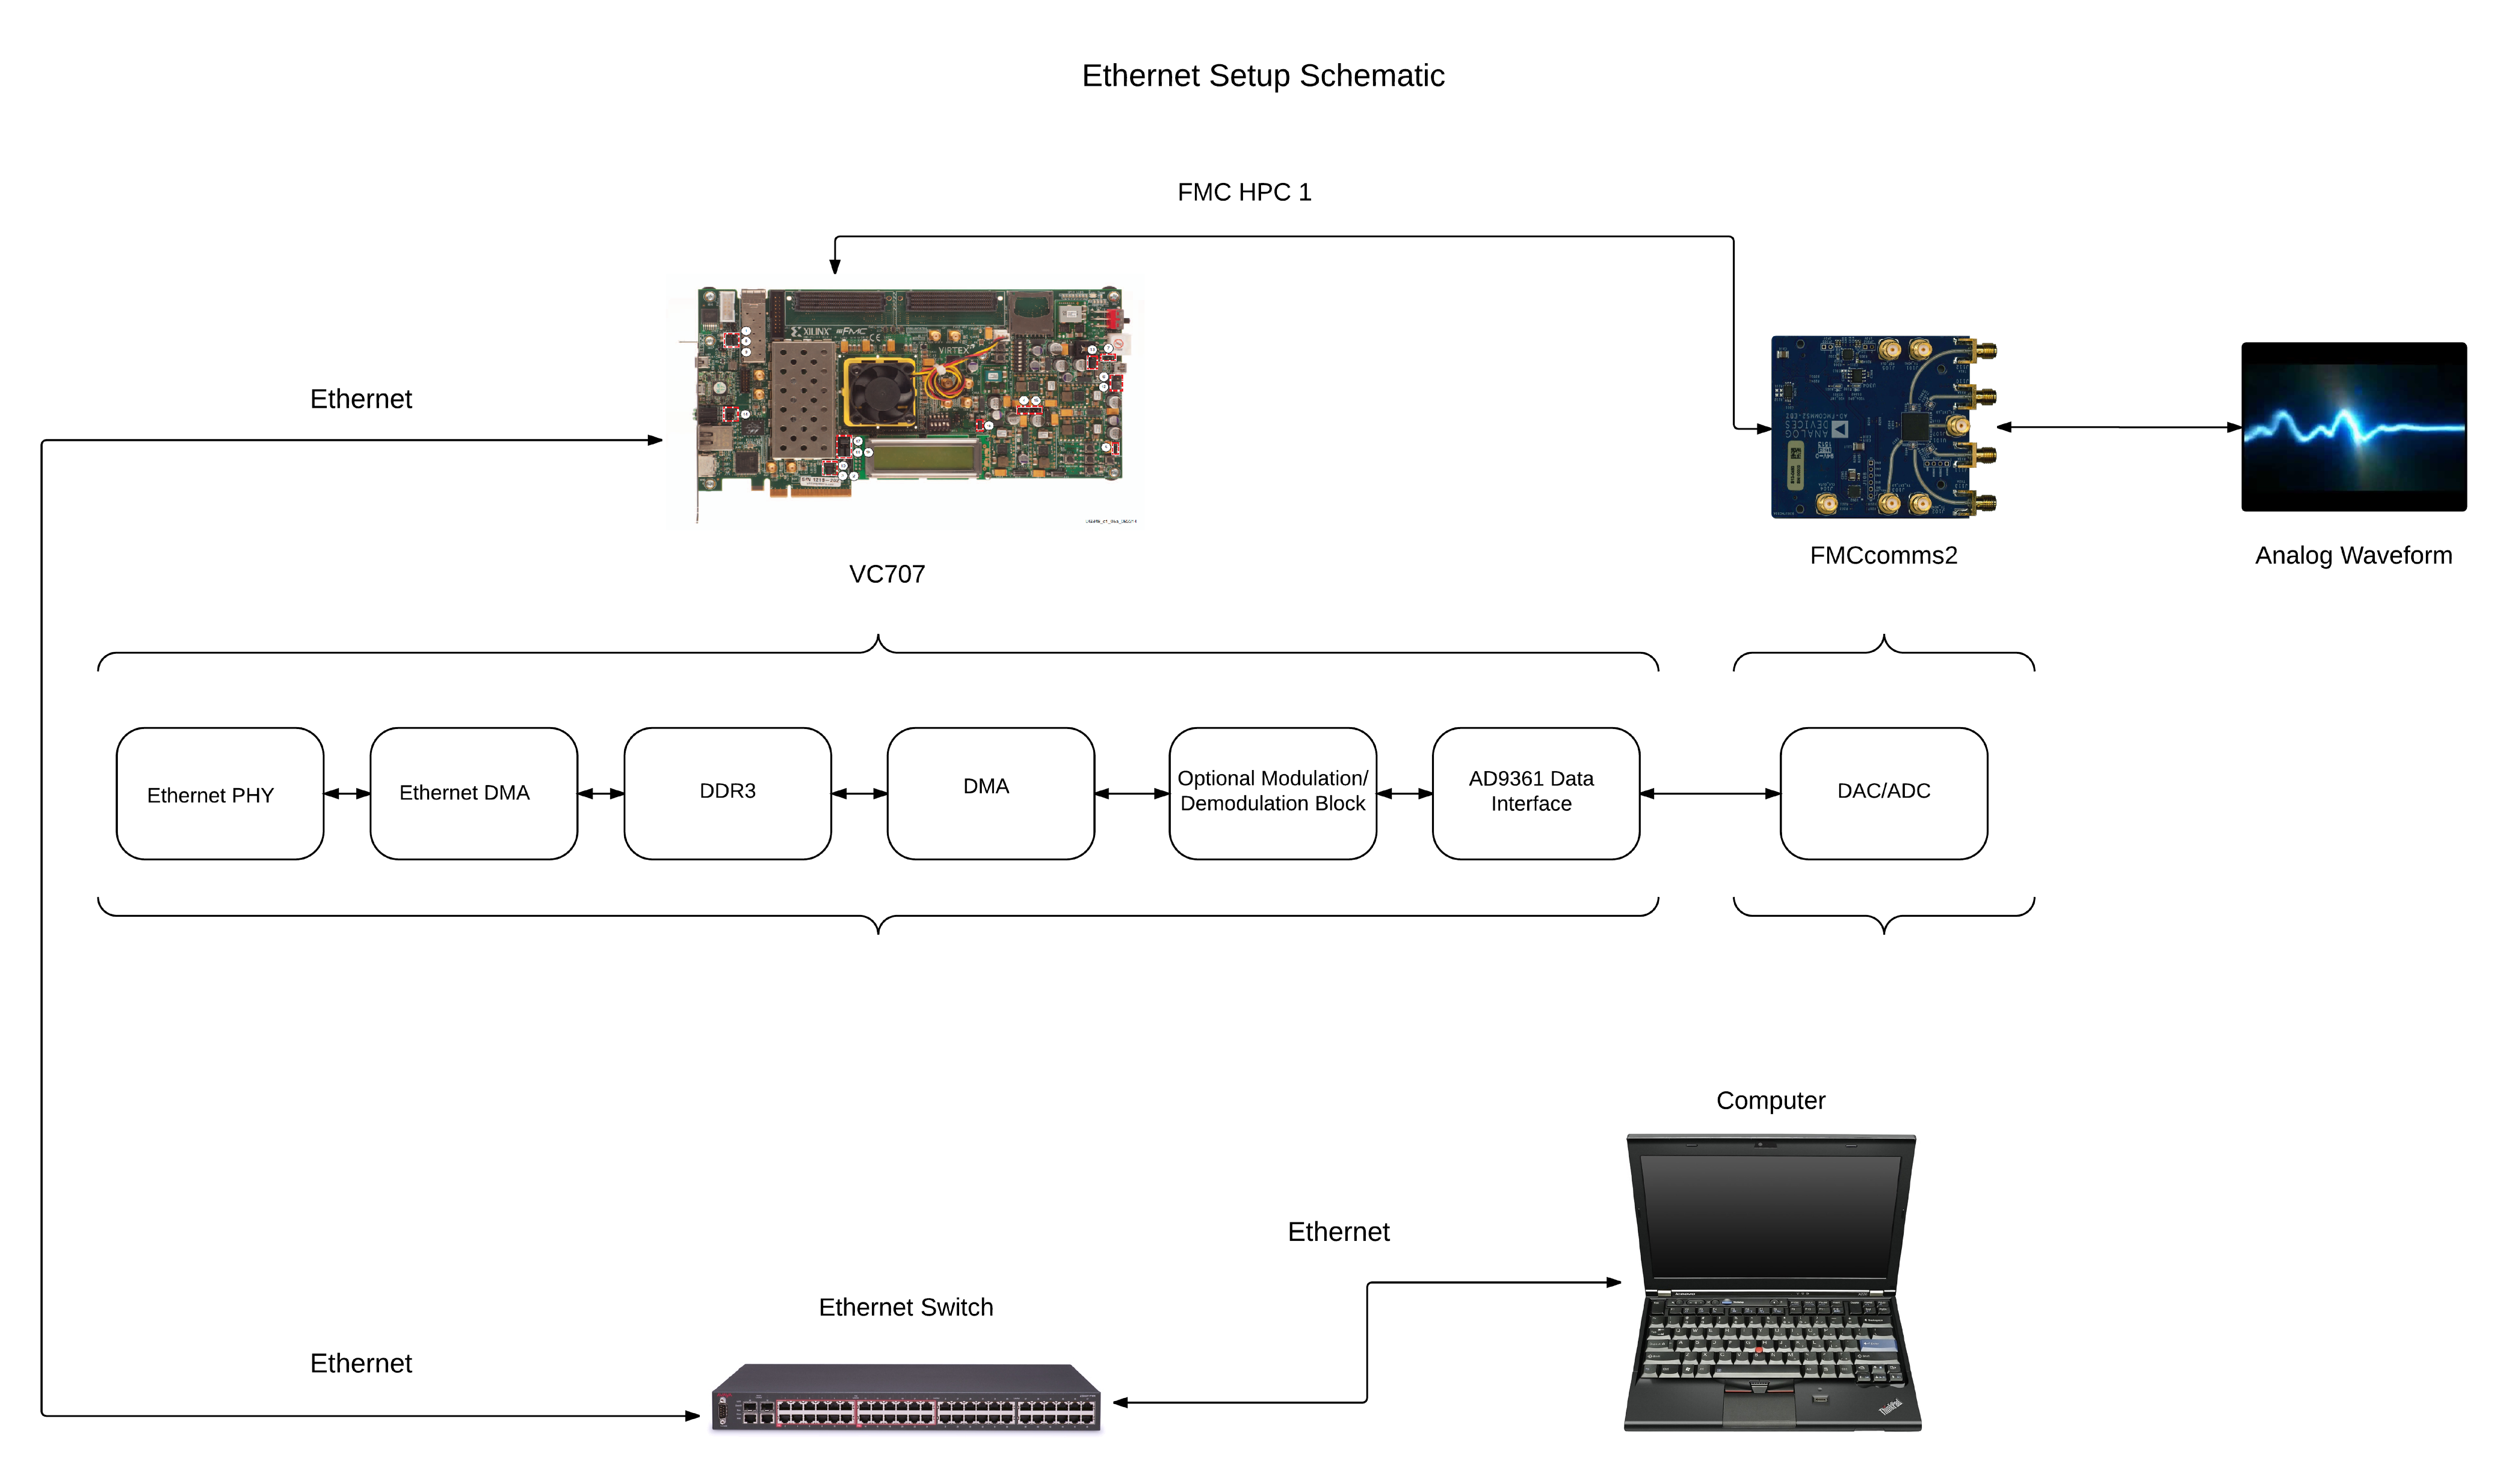
\includegraphics[width=0.65\textwidth]{./figures/eth_setup}
    \caption{ Setup Enhanced with Ethernet Connection
    \label{fig:setupeth}}
\end{figure}
